\section{Analiza performanței}

În această secțiune, vom analiza performanța funcției hash propuse.
Criteriile de analiză for vi multiple, și vor include și comparația cu alte funcții propuse.
Intenția este aceea de a demonstra că funcția hash propusă îndeplinește toate proprietățile de securitate necesare.
Mai mult de atât, vom arăta că funcția hash propusă este și eficientă din punct de vedere computațional spre deosebire de alte funcții hash similare.
Pentru a putea efectua o comparație corectă, am ales următorii parameterii pentru testare:
\begin{itemize}
    \item Dimensiunea hash-ului $l=128$ biți
    \item Dimensiunea blocurilor absorbite de construcția Sponge este de 16 kilobytes.
    \item Numărul maxim de copii în arborele Merkle este de 8.
\end{itemize}

\subsection{Sensibilitatea la mesaj}
Pentru a demonstra sensibilitatea funcției hash propuse la modificări minime aplicate asupra mesajului considerăm următorul mesaj inițial:
\begin{center}
    M0 - "Timpul petrecut cu pisici nu este niciodată irosit."
\end{center}
Ulterior, considerăm 5 variante ale acestui mesaj, fiecare având câte o diferență față de mesajul inițial:
\begin{enumerate}
	\item M1 - i din "pisici" este schimbat cu a
	\item M2 - t din "petrecut" este schimbat cu T
	\item M3 - punctul final este schimbat cu spațiu
	\item M4 - spațiul după "pisici" este schimbat cu !
	\item M5 - i este adăugat la începutul cuvântului "irosit"
\end{enumerate}

\begin{figure}[!htbp]
    \centering
    
\includegraphics[width=\textwidth]{images/test-sensitivity.png}
    \caption{Reprezentarea binară a valorilor hash pentru mesajele M0-M5}
    \label{fig:sensibilitate}
\end{figure}

\newpage

Rezultatul funcției hash pentru fiecare mesaj este prezentat în tabelul de mai jos:

\begin{table}[!htbp]
    \centering
    \begin{tabular}{|c|l|c|}
        \hline
        \textbf{Mesaj} & \textbf{Valoarea hash} & \textbf{Biți modificați (\%)} \\
        \hline
        M0 & \texttt{c339b29bf9b40d20411122e2d5308ac0} & --- \\
        \hline
        M1 & \texttt{f015748b7c3f841a06089ec8682b4f05} & 46.09 \\
        \hline
        M2 & \texttt{bf3898a5f863df303ec9518495153dfc} & 46.88 \\
        \hline
        M3 & \texttt{f94535f32c2cf7467a3b83631f1c6742} & 48.44 \\
        \hline
        M4 & \texttt{6f92c34ef07f7410370c4edaa92a0e26} & 49.22 \\
        \hline
        M5 & \texttt{470ac0a6c76f34b6e1c61bd0e959d97e} & 52.34 \\
        \hline
    \end{tabular}
    \caption{Sensibilitatea la mesaj}
    \label{tab:sensibilitate}
\end{table}

\subsection{Confuzie și difuzie}
Confuzia și difuzia sunt două principii fundamentale de proiectare a sistemelor criptografice, introduse de Shannon~\cite{shannon1949} în contextul sistemelor criptografice.
Confuzia urmărește să facă relația dintre intrare și ieșire cât mai complexă și mai greu de analizat.
Difuzia urmărește disiparea structurii statistice a intrării asupra întregii ieșiri.
Astfel, fiecare bit al ieșirii depinde de cât mai mulți biți ai intrării~\cite{shannon1949}.
Deși au fost formulate inițial pentru cifruri, aceste două criterii au fost adoptate ulterior ca proprietăți esențiale pentru orice primitivă criptografică, inclusiv pentru funcțiile hash.
În cazul unei funcții hash, scopul confuziei și al difuziei este de a îndepărta orice corelație statistică dintre mesajul de intrare și valoarea hash rezultată.
În consecință, o modificare minimă a mesajului produce o valoare hash aparent fără nicio legătură cu cea inițială. \\

Modalitatea de testare a funcției hash este următoarea: se generează un set de $N$ mesaje aleatorii, de lungime aleatoare.
Pentru fiecare mesaj se calculează hash-ul, se schimbă un bit ales arbitrar din mesajul inițial și se calculează hash-ul si pentru mesajul modificat.
Se calculează distanța Hamming dintre cele două hash-uri și se notează această valoare cu $B_i, \forall i \in \overline{1,N}$.
Ulterior, se definesc următoarele metrici pentru fiecare test:

\begin{enumerate}
    \item Numărul mediu de biți modificați:
    \begin{equation}
        B_{med} = \frac{1}{N} \sum_{i=1}^{N} B_i
    \end{equation}

    \item Numărul minim de biți modificați:
    \begin{equation}
        B_{\min} = \min \left\{ B_i \mid i \in \overline{1,N} \right\}
    \end{equation}

    \item Numărul maxim de biți modificați:
    \begin{equation}
        B_{\max} = \max \left\{ B_i \mid i \in \overline{1,N} \right\}
    \end{equation}

    \item Probabilitatea medie de modificare a biților:
    \begin{equation}
        P = \frac{B_{med}}{l} \cdot 100\%
    \end{equation}

    \item Abaterea standard a numărului de biți modificați:
    \begin{equation}
        \Delta B = \sqrt{\frac{1}{N-1} \sum_{i=1}^{N} \left( B_i - B_{med} \right)^2}
    \end{equation}

    \item Abaterea standard a probabilității de modificare:
    \begin{equation}
        \Delta P = \sqrt{\frac{1}{N-1} \sum_{i=1}^{N} \left( \frac{B_i}{l} - P \right)^2} \times 100\%
    \end{equation}
\end{enumerate}

Rezultatele obținute pentru diferite valori ale numărului de teste $N$ sunt prezentate în tabelul de mai jos:

\begin{table}[!htbp]
    \centering
    \begin{tabular}{|c|c|c|c|c|c|c|}
        \hline
        $N$ & $B_{med}$ & $B_{\min}$ & $B_{\max}$ & $P$ (\%) & $\Delta B$ & $\Delta P$ (\%) \\
        \hline
        1000  & 64.0420 & 46 & 84 & 50.0328 & 5.7768 & 4.5131 \\
        \hline
        2500  & 63.9260 & 43 & 86 & 49.9422 & 5.6045 & 4.3785 \\
        \hline
        5000  & 64.0060 & 44 & 85 & 50.0047 & 5.7832 & 4.5181 \\
        \hline
        7500  & 64.0007 & 43 & 87 & 50.0005 & 5.5848 & 4.3631 \\
        \hline
        10000 & 64.0771 & 42 & 85 & 50.0602 & 5.6502 & 4.4142 \\
        \hline
    \end{tabular}
    \caption{Statisticile de confuzie și difuzie pentru valori diferite ale numărului de teste $N$}
    \label{tab:confuzie-difuzie}
\end{table}

\newpage

\begin{figure}[!htbp]
    \centering
    
\includegraphics[width=\textwidth]{images/test-confusion-diffusion-spread.png}
    \caption{Numărul de biți modificați pentru fiecare $B_i$, cu $N=10000$}
    \label{fig:confuzie-difuzie-spread}
\end{figure}

\begin{figure}[!htbp]
    \centering
    
\includegraphics[width=\textwidth]{images/test-confusion-diffusion-spread-histogram.png}
    \caption{Histograma numărului de biți modificați pentru $N=10000$}
    \label{fig:confuzie-difuzie-histograma}
\end{figure}

În mod ideal, pentru o funcție hash cu proprietăți de confuzie și difuzie bune, valoarea numărului mediu de biți modificați $B_{med}$ ar trebui să tindă spre $\frac{l}{2}$.
Conform rezultatelor obținute, se observă că $B_{med}$ este foarte aproape de 64, ceea ce reprezintă exact jumătate din lungimea hash-ului $l=128$ biți.
Valorile lui $\Delta B$ și $\Delta P$ indică faptul că numărul de biți modificați este grupat aproape de valoarea medie.
Conform histogramei \ref{fig:confuzie-difuzie-histograma}, se observă că valorile se încadrează într-o distribuție normală (linia roșie).
În mod similar, conform graficului \ref{fig:confuzie-difuzie-spread}, se observă că numărul de biți modificați variază aleator în vecinătatea valorii medii.

\subsection{Rezistența la coliziuni}
O coliziune apare atunci când două mesaje distincte $M \neq M'$ produc aceeași valoare hash, adică $h(M) = h(M')$.
Rezistența la coliziuni este una dintre proprietățile fundamentale ale unei funcții hash criptografice.
Această caracteristică garantează că este dificil din punct de vedere computațional să se găsească o astfel de pereche de mesaje.
Deoarece o funcție hash comprimă mesaje de lungime arbitrară într-o valoare de lungime fixă de $l$ biți, spațiul intrărilor este mult mai mare decât cel al ieșirilor.
Conform principiului cutiei lui Dirichlet, existența coliziunilor este, prin urmare, inevitabilă.
Rezistența la coliziuni nu înseamnă că funcția hash nu are coliziuni, ci doar că acestea sunt practic imposibil de găsit.
Pornind de la paradoxul zilei de naștere, se poate demonstra că, pentru o funcție hash de $l$ biți, sunt necesare aproximativ $2^{l/2}$ operații de calcul al hash-ului pentru a găsi o coliziune.
Pentru ca un astfel de atac să rămână infezabil în practică, lungimea valorii hash trebuie să fie suficient de mare.
De aceea, în cazul de față am ales $l=128$ biți, ceea ce ridică dificultatea atacului la ordinul a $2^{64}$ operații.
Relevanța acestei cerințe este subliniată de rezultatele relativ recente de criptanaliză, care au demonstrat vulnerabilități în funcții hash consacrate, precum MD5 și SHA-1.
Întrucât funcțiile hash bazate pe sisteme dinamice haotice operează cu numere reale, o demonstrație matematică riguroasă a rezistenței la coliziuni este dificil de realizat. \\

Modalitatea de evaluare a rezistenței la coliziuni hash următoarea: se generează un set de $N$ mesaje aleatorii, de lungime aleatoare.
Pentru fiecare mesaj $M$ se calculează hash-ul, se schimbă un bit ales arbitrar din mesajul inițial obținându-se $M'$.
Se calculează hash-ul si pentru mesajul modificat și se calculează numărul de bytes egali între cele două hash-uri.
În plus, se calculează și suma diferențelor absolute a bytes-ilor celor două hash-uri după formula:

\begin{equation}
    D_i = \sum_{j=1}^{l/8} \abs{Dec(h(M)_j) - Dec(h(M_i)_j)}
\end{equation}

Considerăm că $Dec(x)$ este conversia din byte în formă zecimală, iar $h(M)_j$ reprezintă $j$-lea byte al hash-ului pentru mesajul $M$.
Astfel, este calculată suma minimă, suma maximă, media sumelor și media sumelor raportată la numărul de bytes al hash-ului.

\newpage

\begin{table}[!htbp]
    \centering
    \begin{tabular}{|c|c|c|c|c|c|c|}
        \hline
        \textbf{Bytes egali} & 0 & 1 & 2 & 3 & 4 & 5 \\
        \hline
        \textbf{Hash-uri} & 9401 & 589 & 10 & 0 & 0 & 0 \\
        \hline
        \textbf{Valori teoretice} & 9393 & 590 & 17 & 0 & 0 & 0 \\
        \hline
    \end{tabular}
    \caption{Distribuția numărului de bytes egali pentru $N=10000$ mesaje}
    \label{tab:coliziuni-bytes}
\end{table}

\begin{figure}[!htbp]
    \centering
    
\includegraphics[width=\textwidth]{images/test-character-collisions.png}
    \caption{Distribuția numărului de bytes egali pentru $N=10000$ mesaje}
    \label{fig:coliziuni-bytes}
\end{figure}

\begin{table}[!htbp]
    \centering
    \begin{tabular}{|c|c|c|c|c|}
        \hline
        $N$ & \textbf{Minim} & \textbf{Maxim} & \textbf{Medie} & \textbf{Medie/byte} \\
        \hline
        1000  & 687 & 2193 & 1365.9250 & 85.3703 \\
        \hline
        5000  & 592 & 2234 & 1365.3423 & 85.3338 \\
        \hline
        10000 & 567 & 2278 & 1364.9053 & 85.3066 \\
        \hline
    \end{tabular}
    \caption{Suma diferențelor absolute a bytes-ilor în funcție de $N$}
    \label{tab:diferenta-bytes}
\end{table}

Valorea teoretică pentru media sumelor diferențelor absolute a bytes-ilor, pentru un hash de lungime $l=128$ biți este 1360.
Astfel, se observă că media sumelor se apropie foarte mult de această valoare teoretică, ceea ce indică o rezistență foarte bună la coliziuni.
În plus, conform tabelului \ref{tab:coliziuni-bytes} și graficului \ref{fig:coliziuni-bytes}, se observă că numărul de colizuni pentru hash-uri este sub numărul teoretic.
În consecință, rezistența la coliziuni a funcției hash propuse este foarte bună.

\subsection{Distribuția valorilor hash}
Una dintre primele forme de atac asupra unei funcții hash este criptanaliza statistică, care exploatează eventualele corelații dintre mesajul de intrare și valoarea hash rezultată.
Pentru a împiedica astfel de atacuri, valorile hash trebuie să fie distribuite cât mai uniform pe întreg spațiul valorilor de ieșire.
Distribuția valorilor trebuie să nu păstreze nicio urmă a structurii statistice a mesajului de intrare.
Modalitatea de a testa distribuția valorilor hash este similară cu cea utilizată pentru testarea confuziei și difuziei.
Se generează un set de $N$ mesaje aleatorii, de lungime aleatoare.
Pentru fiecare mesaj $M$ se calculează hash-ul, se schimbă un bit ales aleatoriu din mesajul inițial obținându-se $M'$.
Se calculează hash-ul si pentru mesajul modificat și se numără ce biți s-au schimbat între $h(M)$ și $h(M')$.

\begin{figure}[!htbp]
    \centering
    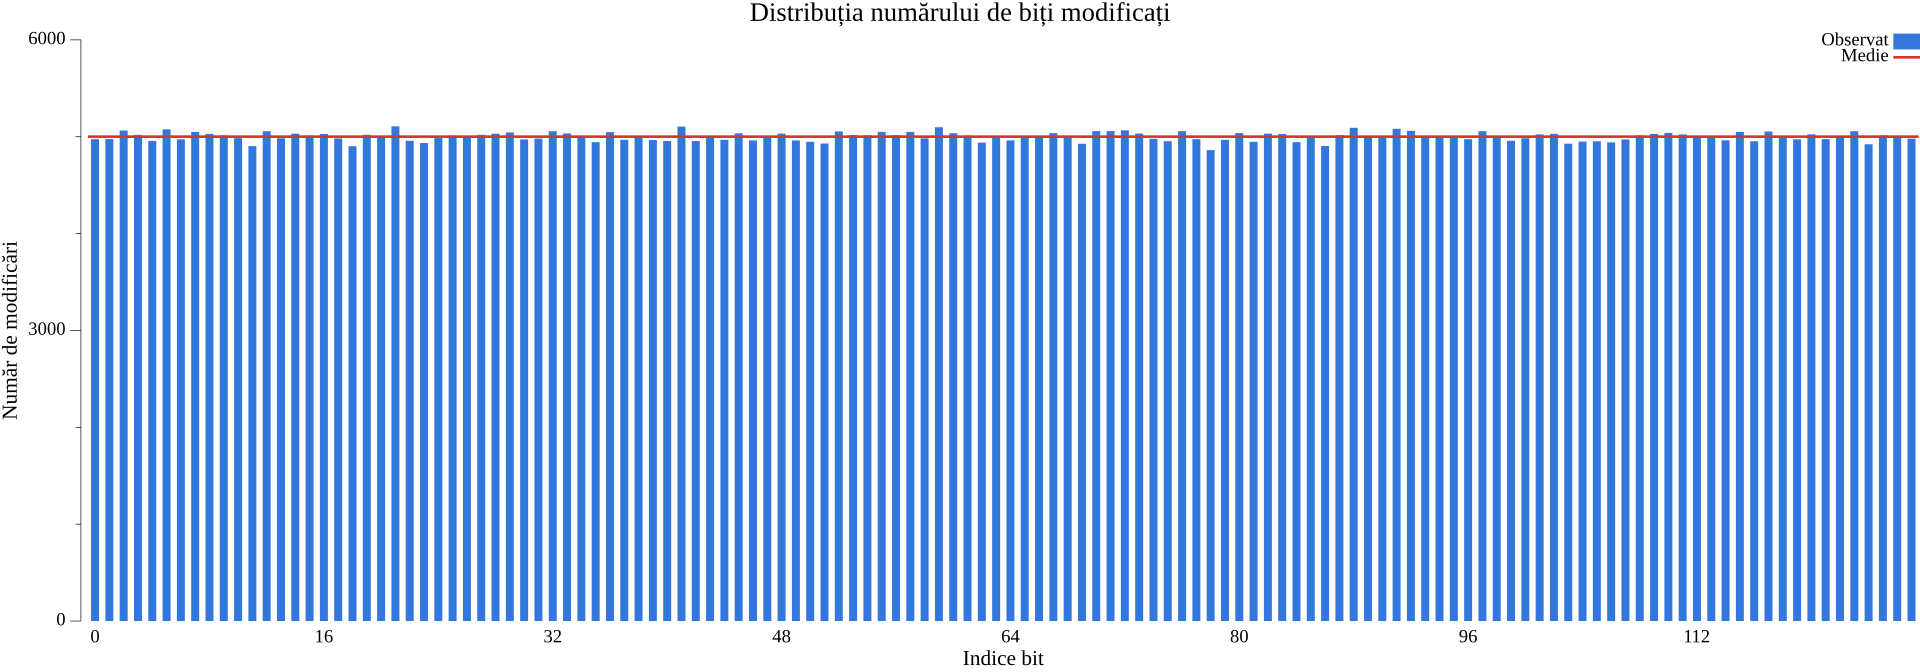
\includegraphics[width=\textwidth]{images/test-changed-bits-distribution.png}
    \caption{Frecvența modificării fiecărui bit al hash-ului pentru $N=10000$ mesaje}
    \label{fig:distributie-valori}
\end{figure}

Valoarea ideală pentru frecvența modificării fiecărui bit al hash-ului este de 50\% din numărul total de teste.
Astfel, pentru $N=10000$ mesaje, fiecare bit al hash-ului ar trebui să se schimbe de aproximativ 5000 de ori.
Conform graficului \ref{fig:distributie-valori}, se observă că frecvența modificării fiecărui bit al hash-ului se apropie foarte mult de această valoare ideală.
Valoarea minimă a frecvenței schimbării unui bit este de 4862, valoarea maximă este de 5107, iar media este de 5000.98.
Aceste rezultate indică faptul că valorile hash sunt distribuite uniform pe întreg spațiul de ieșire.

\subsection{Flexibilitate}
Având în vedere utilizarea construcției Sponge și a arborelui Merkle, funcția hash propusă admite o dimensiune a hash-ului final configurabilă.
Din punct de vedere teoretic, dimensiunea hash-ului poate fi de lungime arbitrară: 128 biți, 192 biți, 256 biți etc.
Numărul de runde intermediare variază în funcție de lungimea hash-ului final, deci pentru același mesaj, hash-urile de lungimi diferite vor fi complet diferite.

\subsection{Eficiența computațională}
Având în vedere că funcția hash propusă utilizează construcția Sponge și arborele Merkle, funcția poate fi ușor paralelizată.
De asemenea, utilizarea operațiilor pe biți, a operațiilor algebrice elementare și a tipurilor de date primitive sporește semnificativ viteza funcției.
Implementarea funcției hash propuse a fost realizată în două limbaje de programare diferite: Go și Rust.
Ambele implementări au fost optimizate pentru performanță, implementarea în Rust obținând viteze cu 30-40\% mai mari decât cea în Go.
Funcția hash propusă a fost testată pe seturi de date de dimensiuni variabile, cu un număr de nuclee alocate variabile.
Testele au fost efectuate pe trei sisteme diferite, cu configurații hardware diferite și cu sisteme de operare diferite:

\begin{itemize}
    \item Mac cu procesor Apple M2 Pro, 16GB RAM și macOS 15.6
    \item Laptop cu procesor AMD Ryzen 7 8845HS, 32GB RAM și Ubuntu 24.04
    \item Desktop cu procesor Intel Xeon Platinum 8370C, 64GB RAM și Windows 11
\end{itemize}